\documentclass{beamer}
\usepackage[utf8]{inputenc}
% \usepackage[english]{babel}
\usepackage{hyperref}
\usepackage{graphicx}
\graphicspath{{../../../output/figures/Presentation/}}
\usepackage{wrapfig}
\usepackage{subcaption}
\usepackage{booktabs,bbm}
% \usepackage[square,numbers]{natbib}
%\bibliographystyle{unsrtnat}

\makeatletter
\let\@@magyar@captionfix\relax
\makeatother
\newtheorem{defn}[theorem]{Definition}
\DeclareMathOperator*{\argmax}{arg\,max}
\DeclareMathOperator*{\argmin}{arg\,min}
\hypersetup{
    allcolors={}
}

\usetheme{Boadilla}
\usecolortheme{beaver}

\usepackage[
backend=biber,
style=bwl-FU,
sorting=ynt
]{biblatex}
\addbibresource{../../main.bib}

\title[Agricultural Index Insurance]{Agricultural Index Insurance: An Optimization Approach}
\author[José Velarde Morales]{José I. Velarde Morales \and Linwei Xin}
\institute[Chicago Booth]
{

  University of Chicago\\
  Booth School of Business

}


\begin{document}
\beamertemplatenavigationsymbolsempty
\frame{\titlepage}
\section{Introduction}

\subsection{The Problem of Agricultural Risk}
\begin{frame}{The Problem of Agricultural Risk}
\begin{itemize}
    \setlength\itemsep{2em}
    \item Farmers face a lot of risk, and the lack of risk management tools forces them to use coping strategies that hurt their long term welfare.
   
    \item Traditional insurance is prohibitively costly in most developing countries due to lack of data and high verification costs.

    \item Moral hazard, adverse selection, and the presence of large covariate shocks make the problem of agricultural insurance especially hard. 
\end{itemize}
\end{frame}

\subsection{A Proposed Solution: Index Insurance}
\begin{frame}{A Proposed Solution: Index Insurance}
\begin{itemize}
   \setlength\itemsep{1em}
    % \item Researchers developed index insurance as a less costly way to offer insurance in developing countries. 
    \item In index insurance, an index (or statistic) is created using easily observable quantities (e.g. rainfall), and it is used to determine whether the insured party suffered an adverse event. 
    \item If the index falls below a pre-determined threshold, the insurance company automatically issues out payments to the insured. 
    \item This allows the insurance company to circumvent the issue of verification and moral hazard, since the actions of individual farmers cannot affect the index.
\end{itemize}
\end{frame}

\begin{frame}{Index Insurance in Practice}
\begin{itemize}
    \setlength\itemsep{1.5em}
    \item Since it was first proposed, index insurance programs have been implemented in many countries including India, Mexico, Tanzania, Malawi, Kenya, and many others (\cite{jensen2017agricultural}). 
    
    \item Today, tens of millions of farmers worldwide are covered by index insurance programs (\cite{greatrex2015scaling}). 
    
    \item However, in most of these cases, the insurance has to be heavily subsidized by governments due to high cost and low demand (\cite{greatrex2015scaling}). 
\end{itemize}
\end{frame}

\subsection{Project Overview}
\begin{frame}{Project Overview}
 \begin{itemize}
    \setlength\itemsep{1em}   
    \item Traditionally, the contract for each insured zone is designed independently of all other zones. %This ignores valuable information about the correlation between zones that affects the cost of insuring the whole portfolio. 
    \item The goal of this project is to make insurance less costly by improving the design of the insurance contracts.
    \item Our method simultaneously determines the contract parameters for different areas, while taking into account the correlation between the areas, reducing risk for the insurer. 
    % \item This allows it to make better trade offs between coverage and the costs associated with risk.
 \end{itemize}
\end{frame}

% \begin{frame}{What I would like feedback on}
%     \begin{itemize}
%        \setlength\itemsep{1em}
%         \item Evaluation (what metrics to report, evaluation with observational and synthetic data, etc.)
%     \end{itemize}
%    \end{frame}

% \subsection{Literature Review}
\begin{frame}{Index Insurance Literature}
 \begin{itemize}
     \item \textbf{Impact of Index Insurance:} Overall, there is evidence that index insurance reduces reliance on detrimental risk-coping strategies, increases investment, and leads to riskier, but more profitable production decisions (\cite{jensen2017agricultural};  \cite{cole2013barriers}; \cite{mobarak2013informal}; \cite{karlan2014agricultural}).
     \item \textbf{Demand for Index Insurance:} Demand for index insurance tends to be low and highly price sensitive (\cite{jensen2017agricultural};  \cite{cole2013barriers}; \cite{cai2020subsidy},\cite{casaburi2018time}).
     \item \textbf{Design of Index Insurance:} There has been relatively little research studying the design of index insurance. The method developed by \cite{chantarat2013designing} is the most commonly used in academic publications (\cite{jensen2019does};  \cite{flatnes2018improving}).
 \end{itemize}
\end{frame}

% \begin{frame}{Optimization Literature}
%  \begin{itemize}
%     \setlength\itemsep{2em}
%      \item We draw from the literature on chance constrained programs (\cite{lagoa2005probabilistically}; \cite{charnes1958cost}).
%      \item  We also draw on the work on coherent risk measures (\cite{artzner1999coherent}), and work on the optimization of conditional value at risk by (\cite{rockafellar2000optimization})
     
%      \item Additionally, we use the results on convex approximations of chance constrained programs by (\cite{nemirovski2007convex}).
%  \end{itemize}
% \end{frame}



\section{Optimization Approach}
\begin{frame}[noframenumbering, plain]
    \frametitle{Content}
    \tableofcontents[currentsection]
  \end{frame}

  
\subsection{Index Insurance Background}
% \begin{frame}{Index Insurance: General Context}
% \begin{itemize}
%     \setlength\itemsep{1em}
%     \item Index insurance is a named-peril insurance.
%     \item It is often tied to access to credit.
%     \item Offered at different levels (micro level, meso level, and macro level)
%     \item Often based on public-private partnerships. Research institutions usually design the product, and insurance companies (or governments) sell it. 
% \end{itemize}
% \end{frame} 

\begin{frame}{Index Insurance: Design}
% Index insurance design generally consists of three steps: 
\begin{enumerate}
    \setlength\itemsep{2em}
    \item Prediction: building a model to predict loss. 
    \item Contract design: designing contracts specifying payouts based on model predictions.
    \item Pricing: product pricing
\end{enumerate}
% This project focuses on the second step. Currently, a research team usually designs the insurance product, and the insurance company then prices the product.
\end{frame} 

\begin{frame}{Index Insurance: Definition and Parameters}
\begin{itemize}
    \setlength\itemsep{1em}
    \item Index insurance uses a signal, $\theta$, to predict agricultural loss, $\hat{\ell}(\theta)$
    \item Contract form: $I(\theta) = \min \left \{ \max \left \{a\hat{\ell}(\theta) - b,0 \right \}, 1 \right \}$, $a,b$ are the contract parameters.
    \item Expected cost for insurer: $C(I(\theta)) = \mathbb{E}[I(\theta)] + c_{\kappa} K(I(\theta))$, where $c_{\kappa}$ is the cost of capital, and $K$ is required capital.
    \item $K(I(\theta)) = CVaR_{1-\epsilon_P}\left ( I(\theta) \right ) - \mathbb{E}[I(\theta)]$.
\end{itemize}
\end{frame}

\begin{frame}{Example of Index Insurance Contract}
    \begin{figure}
        \centering
        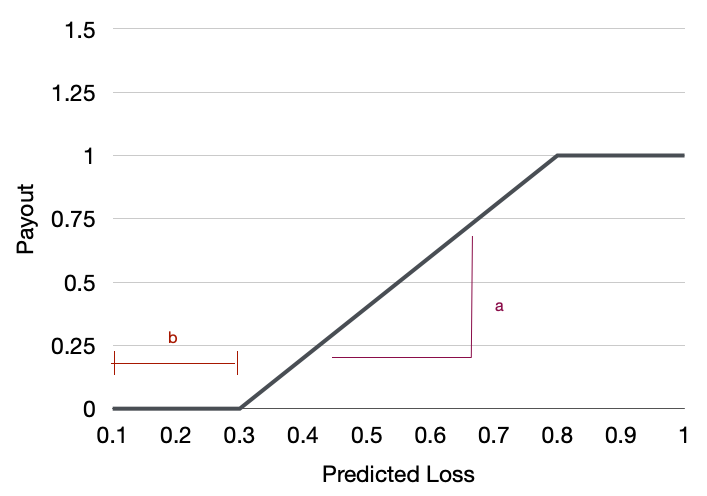
\includegraphics[width=0.9\textwidth]{../../../output/figures/Presentation/sample_insurance_contract.png}
    \end{figure}
\end{frame}

\subsection{Objectives and Constraints}
\begin{frame}{Practitioner Interviews}
\begin{itemize}
   \setlength\itemsep{2em}
    \item We conducted interviews with researchers and practitioners that had implemented index insurance programs in several countries (Malawi, Kenya, Senegal, Thailand, among others) to learn more about the context. 
    \item \textbf{Objective:} minimize risk faced by farmers
    \item \textbf{Constraints:} Price constraints and payout frequency
\end{itemize}    
\end{frame}


\begin{frame}{Risk Measures}
% We are interested in minimizing the risk faced by farmers, so we need a measure of this risk. 

\begin{defn}
    For a random variable $z$, representing loss, the $(1-\epsilon)$ Value at Risk $(VaR)$ is given by 
    \begin{align*}
      VaR_{1-\epsilon}(z) := \inf \left \{ t : P(z \leq t) \geq 1-\epsilon \right \}
    \end{align*}
  \end{defn}

  \begin{defn}
    For a random variable $z$, representing loss, the $(1-\epsilon)$ Conditional Value at Risk $(CVaR)$ is given by 
    \begin{align*}
      CVaR_{1-\epsilon}(z) := \mathbb{E}\left [z | z \geq VaR_{1-\epsilon}(z) \right ]
    \end{align*}
  \end{defn}
\end{frame}

\subsection{CVaR Model}
\begin{frame}{Idealized CVaR Model}
\label{ideal-model}
% \begin{itemize}
%     \item \textbf{Objective:} conditional value at risk of the farmers' loss net of insurance.
%     \item  \textbf{Constraint 1:} piecewise linear structure of the contract. 
%     \item \textbf{Constraint 2:} definition of premium
%     \item \textbf{Constraint 3:} definition of required capital
%     \item \textbf{Constraint 4:} payout frequency constraint
% \end{itemize}
 
\begin{align}
    \min_{a,b,\pi, K}  & \quad {\sf CVaR}_{1-\epsilon}\left ( \ell + \pi - I(\theta) \right ) \nonumber \\
    \text{s.t.} & \quad I(\theta) =  \min \left \{\max \left \{0,a\hat{\ell}(\theta) - b \right \}, 1 \right \}\\
    & \quad \pi = \mathbb{E}\left [ I(\theta) \right ] + c_{\kappa} K \\
    & \quad K = {\sf CVaR}_{1-\epsilon_K}\left ( I(\theta)\right )  - \mathbb{E}[I(\theta)] \\
    & \quad \underline{f} \leq \mathbb{P}\left ( I(\theta) > 0 \right ) \leq \overline{f}\\
    &\quad \pi \leq \overline{\pi}.
\end{align}
\end{frame}

\begin{frame}[noframenumbering]{Idealized CVaR Model}
    \label{ideal-model}
    \begin{align}
        \min_{a,b,\pi, K}  & \quad {\sf CVaR}_{1-\epsilon}\left ( \ell + \pi - I(\theta) \right ) \nonumber \\
        \text{s.t.} & \quad I(\theta) =  \min \left \{\max \left \{0,a\hat{\ell}(\theta) - b \right \}, 1 \right \}\\
        & \quad \pi = \mathbb{E}\left [ I(\theta) \right ] + c_{\kappa} K \\
        & \quad K = {\sf CVaR}_{1-\epsilon_K}\left ( I(\theta)\right )  - \mathbb{E}[I(\theta)] \\
        & \quad \underline{f} \leq \mathbb{P}\left ( I(\theta) > 0 \right ) \leq \overline{f}\\
        &\quad \pi \leq \overline{\pi}.
    \end{align}
    \end{frame}

\begin{frame}{Multiple Zone}
    \begin{align}
        \min_{a,b,K} \max_z &\quad {\sf CVaR}_{1-\epsilon}\left (\ell_z  + \pi_z - I_z(\theta_z) \right )\\
        \text{s.t.   } &\quad I_z(\theta_z) = \min \left \{ \max \left \{ a_z\hat{\ell_z}(\theta_z) + b_z,0 \right \},1 \right \} \\
        &\quad \pi_z  = \mathbb{E}\left [ I_z(\theta_z) \right ] + \frac{c_{\kappa}}{\sum_z s_z} K\\
        &\quad K =  {\sf CVaR}_{1-\epsilon_K} \left ( \sum_z s_z I_z(\theta_z) \right ) - \mathbb{E}\left [ \sum_z s_zI_z(\theta_z) \right ] \\
        & \quad \underline{f} \leq \mathbb{P}\left ( I_z(\theta_z) > 0 \right ) \leq \overline{f}\\
        &\quad\pi_z \leq \overline{\pi_z}
      \end{align}
\end{frame}

\begin{frame}[noframenumbering]{Multiple Zone}
    \begin{align}
        \min_{a,b,K} \max_z &\quad {\sf CVaR}_{1-\epsilon}\left (\ell_z  + \pi_z - I_z(\theta_z) \right )\\
        \text{s.t.   } &\quad I_z(\theta_z) = \min \left \{ \max \left \{ a_z\hat{\ell_z}(\theta_z) + b_z,0 \right \},1 \right \} \\
        &\quad \pi_z  = \mathbb{E}\left [ I_z(\theta_z) \right ] + \frac{c_{\kappa}}{\sum_z s_z} K\\
        &\quad K =  {\sf CVaR}_{1-\epsilon_K} \left ( \sum_z s_z I_z(\theta_z) \right ) - \mathbb{E}\left [ \sum_z s_zI_z(\theta_z) \right ] \\
        & \quad \underline{f} \leq \mathbb{P}\left ( I_z(\theta_z) > 0 \right ) \leq \overline{f}\\
        &\quad\pi_z \leq \overline{\pi_z}
      \end{align}
\end{frame}

\begin{frame}{Convex Relaxation}

    \begin{align}
        \min_{a,b,K,\pi} \max_z &\quad {\sf CVaR}_{1-\epsilon}\left (\ell_z  + \pi_z - \underline{I_z(\theta_z)} \right )\\
        \text{s.t.} &\quad \pi_z  = \mathbb{E}\left [ \overline{I_z(\theta_z)} \right ] + \frac{c_{\kappa}}{\sum_z s_z} K \\
        &\quad K =  {\sf CVaR}_{1-\epsilon_K} \left ( \sum_z s_z\overline{I_z(\theta_z)} \right ) - \mathbb{E}\left [ \sum_z s_z\underline{I_z(\theta_z)} \right ] \\
        & \quad a\hat{\ell_{\underline{f}}} \leq b \leq a\hat{\ell_{\overline{f}}}\\
        &\quad \overline{I_z(\theta_z)} = \max \left \{0,a_z\hat{\ell_z}(\theta_z) + b_z \right \} \\
        &\quad\underline{I_z(\theta_z)} = \min \left \{a_z\hat{\ell_z}(\theta_z)+b_z,1 \right \} \\
        &\quad\pi_z \leq \overline{\pi_z} \nonumber.
      \end{align}
% \hyperlink{ideal-model}{\beamerbutton{Idealized model}}\\
% \hyperlink{convex-approx}{\beamerbutton{Convex approximations}}
\end{frame}

\begin{frame}{LP Reformulation}
\scalebox{0.7}{\parbox{\linewidth}{%
Using the results from \cite{rockafellar2002conditional}, we get: 
\begin{align*}
    \min_{a,b,\alpha,\omega,\gamma,t,m,K,\pi} \quad & m\\
    \text{s.t.} \quad t_z &+ \frac{1}{\epsilon} \sum_j p^j \gamma_z^j \leq m, \forall z\\
    \gamma_z^j &\geq s_z \left (\ell^j + \pi_z - \omega^j_z \right ) -t_z, \forall j, \forall z \\
    \gamma_z^j &\geq 0, \forall j, \forall z\\
    \pi_z &= \frac{1}{N} \sum_j \alpha^j_z + \frac{1}{\sum_z s_z} c_{\kappa} K\\
    t_K &+ \frac{1}{\epsilon_K} \sum_j p^j \gamma_K^j \leq K+ \frac{1}{N}\sum_j \sum_z s_z \omega^j_z\\
    \gamma_K^j &\geq \sum_z s_z \alpha^j_z -t_K, \forall j \\
    \gamma_K^j &\geq 0, \forall j\\
    \alpha^j_z &\geq a_z \hat{\ell_z}(\theta^j_z) + b_z, \forall j, \forall z\\
    \alpha^j_z &\geq 0, \forall j, \forall z\\
    \omega^j_z &\leq a_z \hat{\ell_z}(\theta^j_z) + b_z, \forall j, \forall z\\
    \omega^j_z &\leq 1, \forall j, \forall z\\
    \pi_z &\leq \overline{\pi_z}, \forall z.
  \end{align*}
    }}
\end{frame}

\section{Evaluation}
\begin{frame}[noframenumbering, plain]
    \frametitle{Content}
    \tableofcontents[currentsection,currentsubsection]
\end{frame}
\subsection{Baseline Method}\label{baseline}
\begin{frame}{Baseline Method}
    Baseline method: \cite{chantarat2013designing}. Common in academic publications, used to design Kenya's IBLI program. Method consists of: 
    \\~~\\
    \begin{enumerate}
        \setlength\itemsep{1em}
        \item Use linear model to predict loss.
        \item Contracts are of the form: $I(\theta) = \min \left \{\max \left \{\hat{\ell}(\theta) - b,0 \right \}, 1 \right \}$. $b$ is chosen to maximize the correlation of payouts and losses. 
    \end{enumerate}
\end{frame}

\subsection{Synthetic Data Evaluation}
\begin{frame}[noframenumbering, plain]
    \frametitle{Content}
    \tableofcontents[currentsection,currentsubsection]
\end{frame}

\begin{frame}{What we wanted to test}
    \begin{itemize}
        \setlength\itemsep{2em}
        \item How is our method's performance affected by errors in the prediction model?
        \item How are costs affected by correlation between zones?
    \end{itemize}
\end{frame}

\begin{frame}{Setup}
    We use a linear prediction model and the following data generating process $\ell_z = \frac{1}{1+e^{f(\theta_z)}}$ with $f(\theta_z)$:
    \\~~\\  
      \begin{itemize}
        \item Linear case: $f(\theta) = \beta \theta + \epsilon$
        \item Nonlinear case: $f(\theta) = \beta_0 + \beta_1 \theta + \beta_2 \theta^2 + \ldots + \beta_n \theta^n+ \epsilon$
      \end{itemize}~\\
      In both cases, $\theta \sim \mathcal{N}((0,0),\Sigma), \epsilon \sim \mathcal{N}(0,\rho I)$. In both cases, $\beta_i$ is drawn randomly. Vary $\rho$ to test effect of correlation.
\end{frame}

\begin{frame}{Simulation Details}
    \begin{enumerate}
        \setlength\itemsep{2em}
        \item Generate training and test samples.
        \item Use training data and model predictions to design contracts using both methods.  
        \item Apply insurance contracts designed by the two methods to farmers in the test set and compare outcomes.
        \end{enumerate}~\\
    We run this 200 times for every scenario we test. 
\end{frame}

\begin{frame}{Performance Metrics}
    For each sample in the test set, we calculate the net loss. Then we calculate the following metrics: 
    \\~~\\
    \begin{table}
        \centering
        \begin{tabular}{|l|l|}
            \hline
            \textbf{Farmer Welfare Measures} & \textbf{Insurer Cost/Risk Measures} \\ \hline
            Conditional Value at Risk (CVaR) & Average Cost                        \\
            Value at Risk (VaR)              & Required Capital                    \\
            Semi-Variance                    &                                     \\ \hline
            \end{tabular}
    \end{table}
\end{frame}

\begin{frame}{Summary of Results}
\begin{itemize}
    \setlength\itemsep{2em}
    \item Our model offers comparable protection at much lower costs 
    \item More robust to prediction errors and correlated losses. 
    \item Adjusts payout strategy depending on correlation. 
\end{itemize}
\end{frame}

\begin{frame}{Farmer Risk and Insurer Costs}
\begin{itemize}
    \item Distribution of farmer loss is similar under both
    \item Cost for insurer is radically different
\end{itemize}
\begin{figure}
\centering
  \begin{subfigure}[b]{0.47\textwidth}
    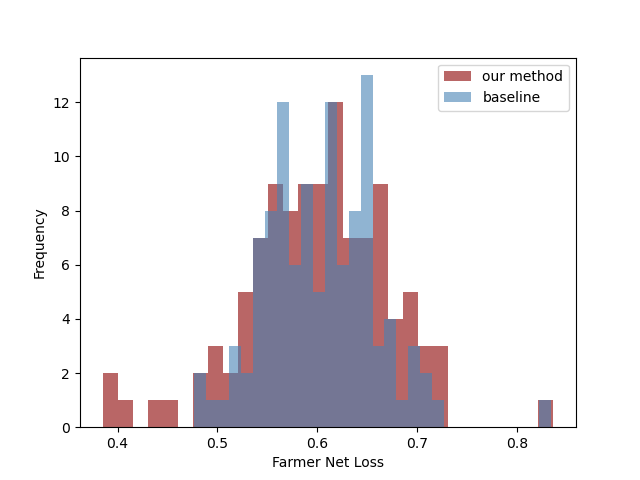
\includegraphics[width=\textwidth]{../../../output/figures/Logit_Bootstrap/farmer_loss_hist_no_corr_linear.png}
    \caption{Farmer net loss}
  \end{subfigure}
 \hfill
  \begin{subfigure}[b]{0.47\textwidth}
    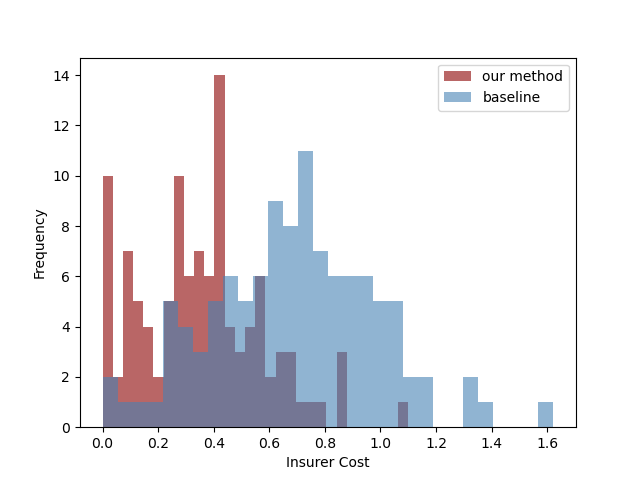
\includegraphics[width=\textwidth]{../../../output/figures/Logit_Bootstrap/insurer_cost_no_corr_linear.png}
    \caption{Insurer cost}
  \end{subfigure}
  \caption{Distribution of outcomes}
\end{figure}
\end{frame}

\begin{frame}{More robust to correlation of losses}
    \begin{figure}
        \centering
        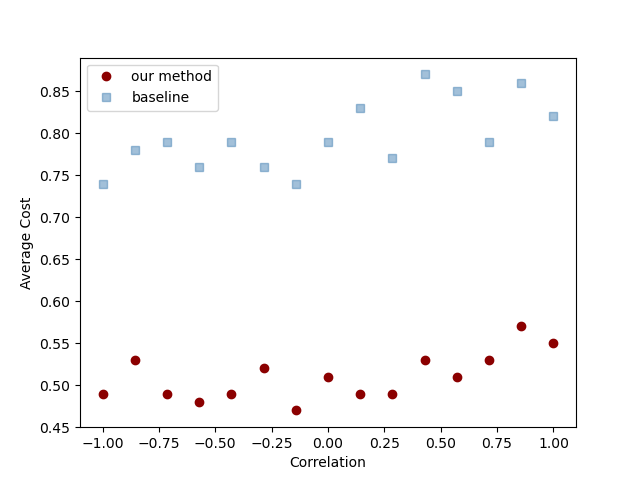
\includegraphics[width=0.9\textwidth]{../../../output/figures/Logit_Bootstrap/cost_vs_corr_linear_exploration.png}
    \end{figure}
\end{frame}

\begin{frame}{More robust to errors in prediction model}
    \begin{figure}
        \centering
          \begin{subfigure}[b]{0.47\textwidth}
            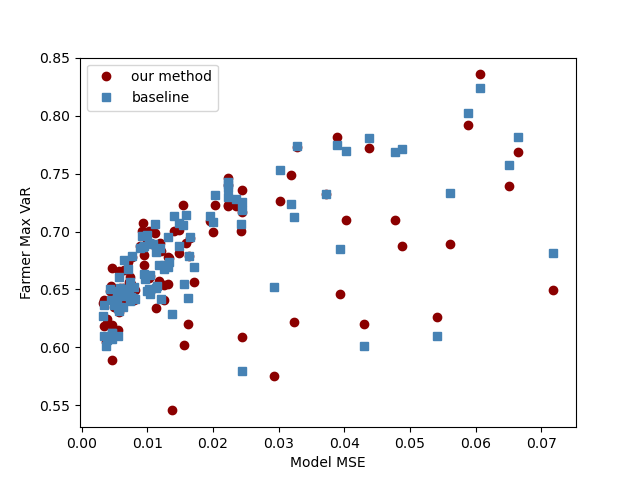
\includegraphics[width=\textwidth]{../../../output/figures/Logit_Bootstrap/Max_VaR_vs_error_nonlinear.png}
            \caption{Farmer VaR}
          \end{subfigure}
         \hfill
          \begin{subfigure}[b]{0.47\textwidth}
            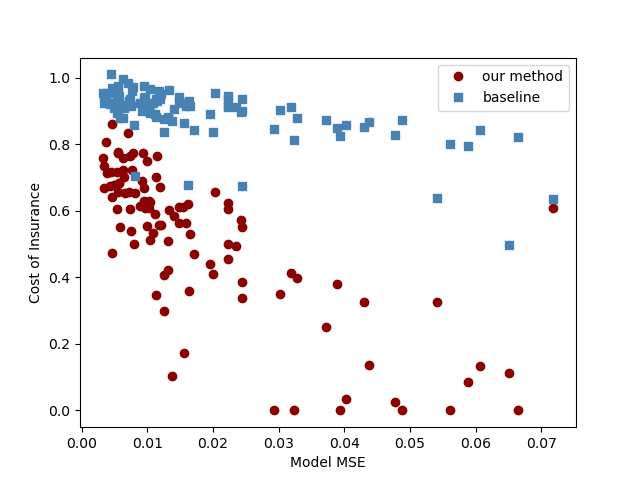
\includegraphics[width=\textwidth]{../../../output/figures/Logit_Bootstrap/cost_vs_error_nonlinear.png}
            \caption{Insurer cost}
          \end{subfigure}
          \caption{Distribution of outcomes}
        \end{figure}
\end{frame}

\begin{frame}{Adjusts payout strategy based on correlation of losses}
\begin{itemize}
    \item Positive correlation leads to smaller but more frequent payouts
    \item Negative correlation leads to less frequent but more aggressive payouts
\end{itemize}
\begin{figure}
\centering
  \begin{subfigure}[b]{0.45\textwidth}
    \includegraphics[width=\textwidth]{../../../output/figures/Presentation/slope_vs_corr.png}
    \caption{Slope of payout function vs correlation}
  \end{subfigure}
 \hfill
  \begin{subfigure}[b]{0.45\textwidth}
    \includegraphics[width=\textwidth]{../../../output/figures/Presentation/intercept_vs_corr.png}
    \caption{Intercept of payout function vs correlation}
  \end{subfigure}
  \caption{Relationship between parameters and correlation}
\end{figure}
    
\end{frame}


% \begin{frame}{Summary of Results: Misspecified Model}
%     In this case, our results are even stronger. We match the performance of the basline method on most metrics, and the cost is significantly lower. 
%     \begin{itemize}
%         \setlength\itemsep{1em}
%         \item \textbf{Metrics on which our model does better:} Maximum Semi-Variance, Required Capital 
%         \item \textbf{Metrics on which baseline model does better:} Maximum CVaR 
%         \item \textbf{Metrics on which we tie:} Maximum VaR, Average Cost
%     \end{itemize} 
%     \end{frame}

%     \begin{frame}{Histograms: Model Misspecified}
%         \begin{itemize}
%             \item Distribution of farmer loss is similar under both
%             \item Cost for insurer is radically different
%         \end{itemize}
%         \begin{figure}
%         \centering
%           \begin{subfigure}[b]{0.47\textwidth}
%             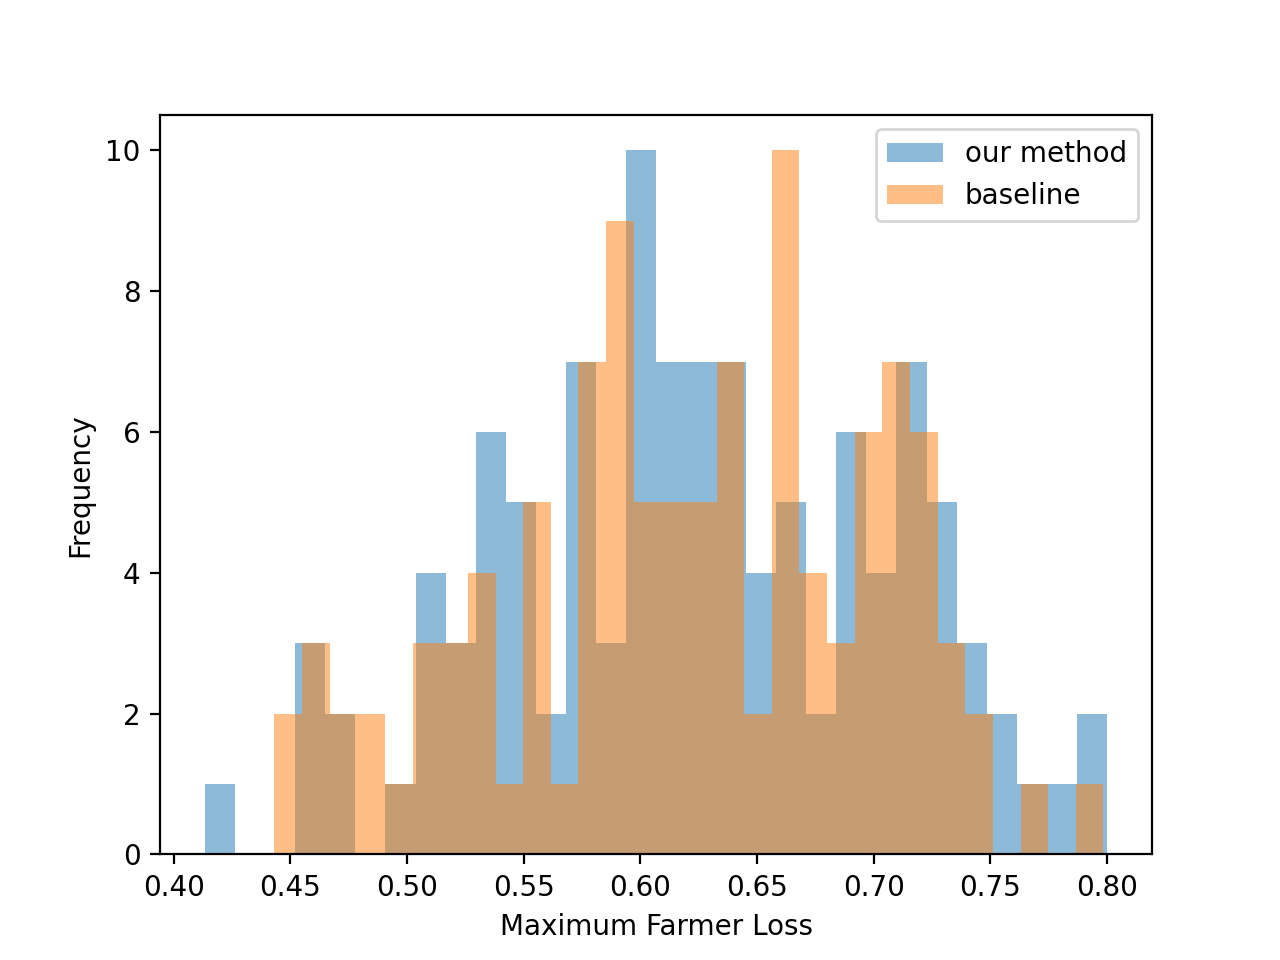
\includegraphics[width=\textwidth]{../../../output/figures/Logit_Bootstrap/farmer_loss_hist_no_corr_nonlinear.png}
%             \caption{Farmer net loss}
%             \label{fig:f1}
%           \end{subfigure}
%          \hfill
%           \begin{subfigure}[b]{0.47\textwidth}
%             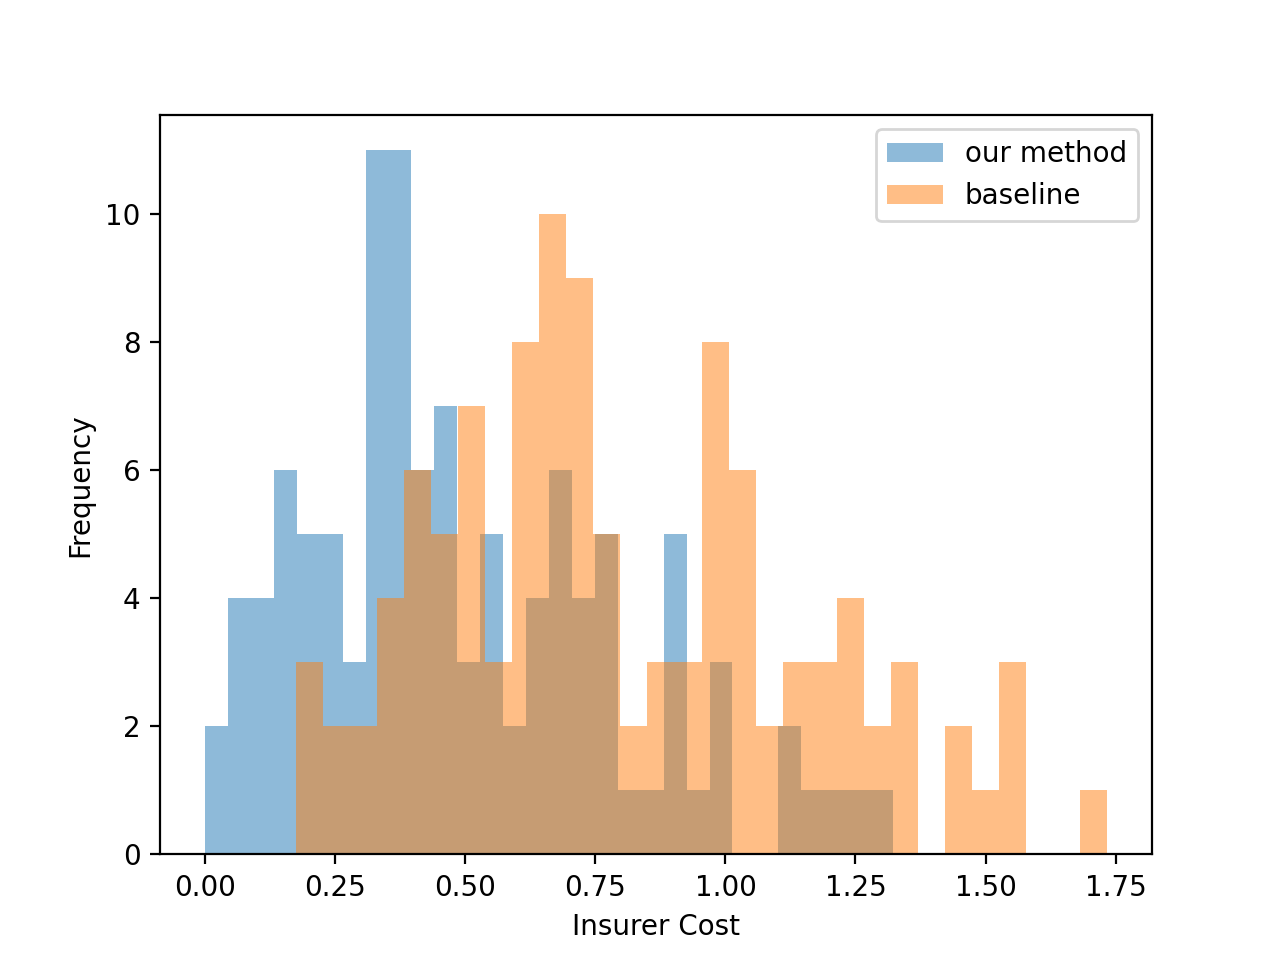
\includegraphics[width=\textwidth]{../../../output/figures/Logit_Bootstrap/insurer_cost_no_corr_nonlinear.png}
%             \caption{Insurer cost}
%             \label{fig:f2}
%           \end{subfigure}
%           \caption{Distribution of outcomes}
%         \end{figure}
            
%         \end{frame}

% \begin{frame}[noframenumbering, plain]{Results: Misspecified Prediction Model}
%     \fontsize{6.5pt}{8pt}\selectfont
%     \begin{table}
%     \subcaptionbox{No correlation}{
%         \begin{tabular}{ccccccc}
%             \toprule
%             Model &     Max CVaR &       Max VaR &   Max SemiVar & $|VaR_2 - VaR_1|$ & Required Capital & Average Cost \\
%          \midrule
%          Baseline &         0.65 &          0.67 &          0.02 &              0.02 &             0.70 &         0.91 \\
%                   &  [0.6, 0.84] &  [0.61, 0.77] &  [0.01, 0.08] &       [0.0, 0.07] &     [0.21, 0.93] &  [0.7, 0.97] \\
%               Opt &         0.71 &          0.67 &          0.03 &              0.02 &             0.61 &         0.56 \\
%                   & [0.64, 0.86] &  [0.61, 0.77] &  [0.01, 0.08] &       [0.0, 0.08] &      [0.0, 0.86] &  [0.0, 0.74] \\
%              Diff &        -0.04 &         -0.00 &         -0.00 &             -0.00 &             0.10 &         0.36 \\
%                   & [-0.1, 0.02] & [-0.02, 0.06] & [-0.03, 0.02] &     [-0.03, 0.03] &    [-0.03, 0.26] & [0.18, 0.81] \\
%          \bottomrule
%             \end{tabular}}
    
%     \subcaptionbox{Positive correlation}{
%         \begin{tabular}{ccccccc}
%             \toprule
%             Model &      Max CVaR &       Max VaR &   Max SemiVar & $|VaR_2 - VaR_1|$ & Required Capital & Average Cost \\
%          \midrule
%          Baseline &          0.68 &          0.69 &          0.02 &              0.01 &             0.98 &         0.95 \\
%                   &  [0.62, 0.85] &  [0.63, 0.79] &  [0.01, 0.05] &       [0.0, 0.04] &     [0.26, 1.21] & [0.59, 1.03] \\
%               Opt &          0.73 &          0.69 &          0.03 &              0.02 &             0.83 &         0.57 \\
%                   &  [0.66, 0.86] &  [0.62, 0.76] &  [0.01, 0.08] &       [0.0, 0.05] &      [0.0, 1.19] &   [0.0, 0.8] \\
%              Diff &         -0.04 &          0.00 &         -0.00 &             -0.00 &             0.13 &         0.36 \\
%                   & [-0.09, 0.01] & [-0.02, 0.07] & [-0.04, 0.01] &     [-0.03, 0.02] &    [-0.07, 0.38] & [0.14, 0.81] \\
%          \bottomrule
%             \end{tabular}}
    
%     \end{table}
%     \end{frame}
    

% \begin{frame}{Relationships between parameters and correlation}
% \begin{itemize}
%     \item Positive correlation leads to smaller but more frequent payouts
%     \item Negative correlation leads to less frequent but more aggressive payouts
% \end{itemize}
% \begin{figure}
% \centering
%   \begin{subfigure}[b]{0.45\textwidth}
%     \includegraphics[width=\textwidth]{slope_vs_corr.png}
%     \caption{Slope of payout function vs correlation}
%     \label{fig:f1}
%   \end{subfigure}
%  \hfill
%   \begin{subfigure}[b]{0.45\textwidth}
%     \includegraphics[width=\textwidth]{intercept_vs_corr.png}
%     \caption{Intercept of payout function vs correlation}
%     \label{fig:f2}
%   \end{subfigure}
%   \caption{Relationship between parameters and correlation}
% \end{figure}
    
% \end{frame}



\subsection{Kenya Pastoralist Data}
\begin{frame}[noframenumbering, plain]
    \frametitle{Content}
    \tableofcontents[currentsection,currentsubsection]
\end{frame}

\begin{frame}{Data Sources}
\begin{itemize}
    \setlength\itemsep{2em}
    \item \textbf{NDVI Data:} The Normalized Difference Vegetation Index (NDVI) is a satellite-based indicator of the amount and health of vegetation. We use NDVI data for Kenya between 2000-2015. %There are $\sim 23,000,000$ observations per time period, and 365 time periods.
    \item \textbf{Kenya Household Survey Data:} This survey was conducted as part of the development of the Index based livestock insurance (IBLI) program in northern Kenya.  This dataset has information on household location, livestock levels and changes for each month in 2010-2013. There are 900 households in this dataset. 
    %\item \textbf{Kenya Geospatial Data:} This dataset contains the geospatial boundaries of larger villages in Kenya. 
\end{itemize}
\end{frame}

% \begin{frame}{Data Creation}
% \begin{enumerate}
%    \item Data for prediction model
%    \begin{enumerate}
%        \item NDVI Data
%        \begin{enumerate}
%         %    \item Change NDVI data coordinates to standard coordinates
%            \item Use geospatial information to merge NDVI data with village geospatial data. 
%            \item For each village, you now have many NDVI values. Use this to calculate village level features for relevant time periods. 
%            \item \textbf{Outcome:} data set with village level NDVI features across time.
%        \end{enumerate}
%        \item Survey Data
%        \begin{enumerate}
%            \item Merge survey data with Kenya geospatial data. 
%            \item Calculate herd mortality for each village in each season. 
%            \item \textbf{Outcome:} data set with village level herd mortality across time
%        \end{enumerate}
%        \item Merge two datasets at the village by season level.
%    \end{enumerate}
%    \item Train prediction model using data from previous step. 
%     \item Add model predictions to household survey data 
% \end{enumerate}
% \begin{enumerate}
%     \item Calculate NDVI metrics for each village in each season. These metrics will be the features for our predictive model. 
%     \item Use household data to calculate average livestock mortality in each village in each season. 
%     \item Merge the two resulting datasets to create a dataset for regression.
%     \item Train prediction model for each cluster and use this model to predict herd mortality at the village level. 
%     \item Add model predictions to household data. 
% \end{enumerate}   
% \end{frame}

\begin{frame}{Evaluation Procedure}
We use leave one out cross validation to evaluate our method. In each iteration, we leave out one year of data for testing.
% \begin{enumerate}
%     \item Split regression data and household survey data into training/test set
%     \item Train prediction model on training data
%     \item Use model to calculate village level predicted losses, add this to household training data
%     \item Calculate insurance contracts based on the training data using both methods.
%     \item Use prediction model to calculate village level predicted losses on the test set. 
%     \item Calculate insurance payouts on test data.
% \end{enumerate}
\begin{enumerate}
    \item Split data into training and test sets 
    \item Use training data and model predictions to design contracts using both methods.
    \item Apply insurance contracts designed by the two methods to farmers in the test set and compare outcomes.
\end{enumerate}
\end{frame}

\begin{frame}{Results}
The insurance contracts developed by our model provide slightly better protection at a much lower cost. The cost of our contracts is $9\%$ lower, and the cost of capital is $13\%$ lower. 
\begin{table}[]
\small
    \centering
%     \begin{tabular}{lrrrr}
% \toprule
%     Model &  Max VaR &  $|VaR_2 - VaR_1|$ &  Required Capital &  Average Cost \\
% \midrule
%  Baseline &     1303 &               1316 &           3014405 &          6449 \\
%       Opt &     1286 &               1361 &           2626260 &          5864 \\
% \bottomrule
% \end{tabular}

\begin{tabular}{lrrrr}
    \toprule
       Model &  Max CVaR &  Max VaR &  $|VaR_2 - VaR_1|$ &  Average Cost \\
    \midrule
    Baseline &      0.69 &     0.52 &               0.13 &       \textbf{5263.64} \\
         Opt &      0.65 &     0.53 &               0.10 &       \textbf{3794.80} \\
    \bottomrule
    \end{tabular}
    \caption{Results using Kenya household data}
    
\end{table}
\end{frame}

\section{Conclusion}
\subsection{Conclusions}
\begin{frame}{Conclusions}
    \begin{itemize}
    \setlength\itemsep{2em}
        \item The contracts designed by our model are able to offer comparable protection at lower costs than the baseline method. 
        \item Our method is able to outperform the baseline because it is more robust to errors in the prediction model. 
        \item Our method is more cost effective because it takes into account spatial correlations between areas to better manage risk. Thus, the model makes better trade offs between costs and coverage than the baseline method. 
    \end{itemize}
\end{frame}

% \subsection{Next Steps}
% \begin{frame}{Next Steps}
% \begin{itemize}
% \setlength\itemsep{2em}
%     \item We are working with practitioners to improve the model and possibly test it in practice.
%     \item We are working with the Bank of Thailand on the implementation of their satellite-based index insurance program. 
%     \item We are also talking to the International Research Institute for Climate and Society at Columbia, they have worked on the implementation of numerous index insurance programs in Africa.   
% \end{itemize}
% \end{frame}

\begin{frame}[noframenumbering, plain]{References}
\footnotesize
\printbibliography
\end{frame}

\begin{frame}[noframenumbering, plain]{Idealized CVaR Model}
% \label{ideal-model}
\begin{itemize}
    \item \textbf{Objective:} conditional value at risk of the farmers' loss net of insurance.
    \item  \textbf{Constraint 1:} piecewise linear structure of the contract. 
    \item \textbf{Constraint 2:} budget constraint.
    \item \textbf{Constraint 3:} definition of required capital.
\end{itemize}
 
\begin{align}
        \min_{a,b,\pi, K}  & \quad CVaR_{1-\epsilon}\left ( \ell - I(\theta) \right ) \notag\\
        \text{s.t.   }I(\theta) &= \min \{ (a\hat{\ell}(\theta) + b)^+,P \} \\
        \mathbb{E}\left [ I(\theta) \right ] &+ c_{\kappa} K \leq B \\
        K &= \left( CVaR_{1-\epsilon}\left ( I(\theta) \right ) - \mathbb{E}[I(\theta)] \right) \label{cons-budget}
    \end{align}
\end{frame}

\begin{frame}[noframenumbering, plain]{The problem is non-convex, so we need convex approximations}
\label{convex-approx}
We use the following approximations of $I(\theta)$ to make the problem convex: 
\begin{align*}
    \overline{I(\theta)} &\triangleq \max \left \{ 0,a\hat{\ell}(\theta) + b\right \} \\
    \underline{I(\theta)} &\triangleq \min \{ a\hat{\ell}(\theta) + b,K \}
\end{align*}
\begin{itemize}
    \item Note that $\overline{I(\theta)} \geq I(\theta)$ and $\overline{I(\theta)}$ is convex. Conversely, $\underline{I(\theta)} \leq I(\theta)$ and $\underline{I(\theta)}$ is concave. 
    \item We replace $I(\theta)$ with either $\overline{I(\theta)}$ or $\underline{I(\theta)}$ where necessary to obtain conservative and convex approximations. 
    \item We also need approximations or proxies for $E[I(\theta)]$ in constraint . We use $\pi_{SQ} = E[I_{SQ}(\theta)]$, where $I_{SQ}$ is the contract designed using the status quo method, as a proxy for $E[I(\theta)]$ in constraint .
\end{itemize}
\end{frame}

\begin{frame}[noframenumbering, plain]{Insights: Relationships between parameters and epsilon}
\label{eps-relationship}
As $\epsilon$ gets smaller, the slope increases and the function shifts to the right. 
\begin{figure}
\centering
  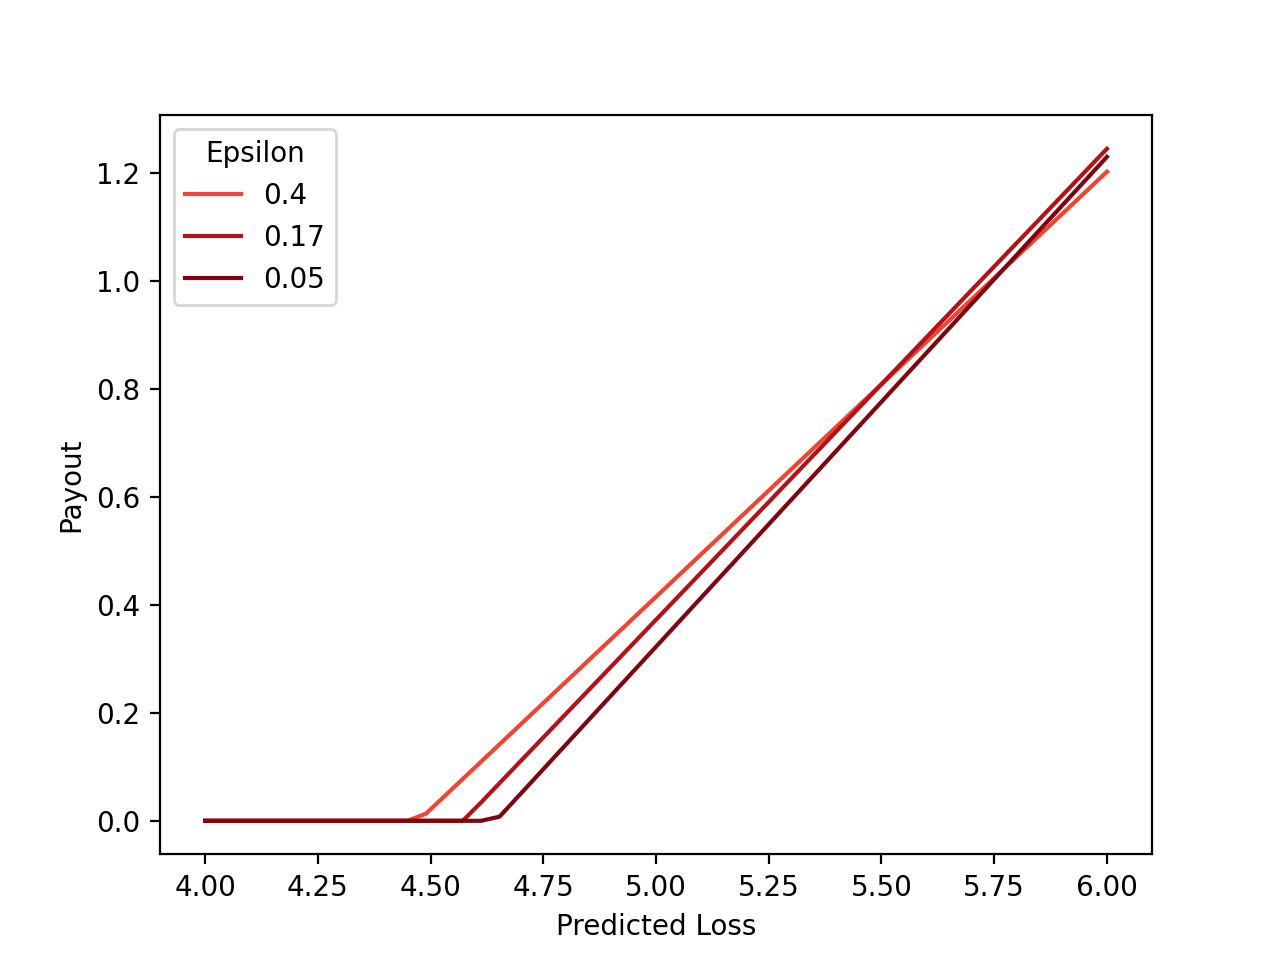
\includegraphics[width=0.65\textwidth, height=0.5\textwidth]{payout_vs_epsilon.png}
\end{figure}
    
\end{frame}

\begin{frame}[noframenumbering, plain]{Results: Misspecified Prediction Model}
\label{misspec-results}
\fontsize{6.5pt}{8pt}\selectfont
\begin{table}
\subcaptionbox{No correlation}{
\begin{tabular}{ccccc}
\toprule
   Model &        Max VaR & $|VaR_2 - VaR_1|$ & Required Capital &   Average Cost \\
\midrule
Baseline &          27.42 &              1.65 &            53.85 &          40.73 \\
         & [25.13, 29.57] &      [0.16, 5.56] &   [44.81, 59.88] & [36.06, 45.83] \\
     Opt &          27.41 &              1.96 &            49.97 &          40.36 \\
         & [24.53, 29.83] &       [0.15, 5.6] &   [42.87, 58.53] &  [35.52, 45.5] \\
\bottomrule
\end{tabular}}

\subcaptionbox{Positive correlation}{
\begin{tabular}{ccccc}
\toprule
   Model &        Max VaR & $|VaR_2 - VaR_1|$ & Required Capital &   Average Cost \\
\midrule
Baseline &          27.16 &              1.23 &             57.1 &          41.36 \\
         &  [24.7, 29.62] &       [0.1, 5.05] &    [51.16, 62.9] & [36.24, 46.52] \\
     Opt &          27.71 &               1.1 &            56.51 &          41.31 \\
         & [24.91, 30.31] &      [0.09, 3.62] &   [50.92, 62.26] & [35.98, 46.82] \\
\bottomrule
\end{tabular}}

\subcaptionbox{Negative correlation}{
\begin{tabular}{ccccc}
\toprule
   Model &        Max VaR & $|VaR_2 - VaR_1|$ & Required Capital &   Average Cost \\
\midrule
Baseline &          27.52 &               1.9 &             25.2 &          36.42 \\
         & [25.09, 29.69] &       [0.17, 6.0] &   [17.99, 36.35] & [33.13, 41.88] \\
     Opt &          27.39 &              1.84 &            26.77 &          36.67 \\
         & [24.33, 29.71] &      [0.16, 5.49] &    [18.17, 37.5] & [33.21, 42.03] \\
\bottomrule
\end{tabular}
}
\end{table}
\end{frame}

\end{document}